\documentclass[runningheads]{llncs}
\usepackage[T1]{fontenc}
\usepackage{tikz}
\usepackage{amsmath}
\usepackage{amssymb}
\usetikzlibrary{decorations.pathreplacing}

\begin{document}

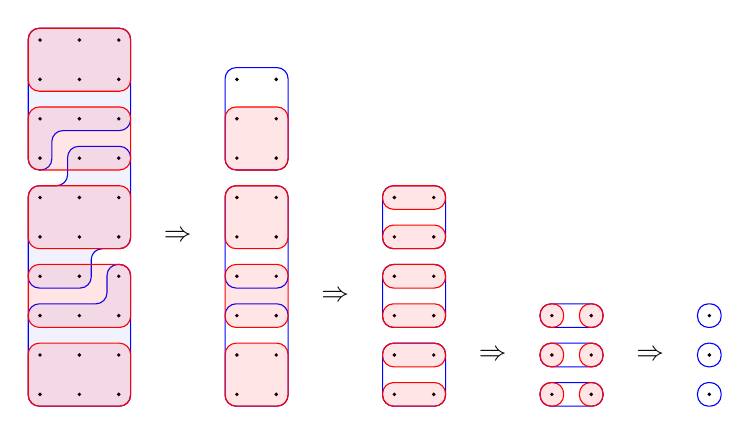
\begin{tikzpicture}
    \foreach \x in {0.25, 0.75, 1.25} {
        \foreach \y in {0.25, 0.75, 1.25, 1.75, 2.25, 2.75, 3.25, 3.75, 4.25, 4.75} {
            \node[circle, fill, inner sep=0.5] at (\x, \y) {};
        }
    }

    \draw[rounded corners, blue, fill, fill opacity=0.05] (0.1, 0.1) -- (1.4, 0.1) -- (1.4, 1.9) --
    (1.1, 1.9) -- (1.1, 1.4) -- (0.1, 1.4) -- cycle;
    \draw[rounded corners, blue, fill, fill opacity=0.05] (0.1, 1.6) -- (0.9, 1.6) -- (0.9, 2.1) --
    (1.4, 2.1) -- (1.4, 3.4) -- (0.6, 3.4) -- (0.6, 2.9) -- (0.1, 2.9) -- cycle;
    \draw[rounded corners, blue, fill, fill opacity=0.05] (0.1, 3.1) -- (0.4, 3.1) -- (0.4, 3.6) --
    (1.4, 3.6) -- (1.4, 4.9) -- (0.1, 4.9) -- cycle;

    \draw[rounded corners, red, fill, fill opacity=0.1] (0.1, 0.1) -- (1.4, 0.1) -- (1.4, 0.9)
    -- (0.1, 0.9) -- cycle;
    \draw[rounded corners, red, fill, fill opacity=0.1] (0.1, 1.1) -- (1.4, 1.1) -- (1.4, 1.9)
    -- (0.1, 1.9) -- cycle;
    \draw[rounded corners, red, fill, fill opacity=0.1] (0.1, 2.1) -- (1.4, 2.1) -- (1.4, 2.9)
    -- (0.1, 2.9) -- cycle;
    \draw[rounded corners, red, fill, fill opacity=0.1] (0.1, 3.1) -- (1.4, 3.1) -- (1.4, 3.9)
    -- (0.1, 3.9) -- cycle;
    \draw[rounded corners, red, fill, fill opacity=0.1] (0.1, 4.1) -- (1.4, 4.1) -- (1.4, 4.9)
    -- (0.1, 4.9) -- cycle;

    \begin{scope}[shift={(0.5, 0)}]
        \foreach \x in {2.25, 2.75} {
            \foreach \y in {0.25, 0.75, 1.25, 1.75, 2.25, 2.75, 3.25, 3.75, 4.25} {
                \node[circle, fill, inner sep=0.5] at (\x, \y) {};
            }
        }

        \draw[rounded corners, blue, fill opacity=0.05] (2.1, 0.1) -- (2.9, 0.1) -- (2.9, 1.4)
        -- (2.1, 1.4) -- cycle;
        \draw[rounded corners, blue, fill opacity=0.05] (2.1, 1.6) -- (2.9, 1.6) -- (2.9, 2.9)
        -- (2.1, 2.9) -- cycle;
        \draw[rounded corners, blue, fill opacity=0.05] (2.1, 3.1) -- (2.9, 3.1) -- (2.9, 4.4)
        -- (2.1, 4.4) -- cycle;

        \draw[rounded corners, red, fill, fill opacity=0.1] (2.1, 0.1) -- (2.9, 0.1) -- (2.9,
        0.9) -- (2.1, 0.9) -- cycle;
        \draw[rounded corners, red, fill, fill opacity=0.1] (2.1, 1.1) -- (2.9, 1.1) -- (2.9,
        1.9) -- (2.1, 1.9) -- cycle;
        \draw[rounded corners, red, fill, fill opacity=0.1] (2.1, 2.1) -- (2.9, 2.1) -- (2.9,
        2.9) -- (2.1, 2.9) -- cycle;
        \draw[rounded corners, red, fill, fill opacity=0.1] (2.1, 3.1) -- (2.9, 3.1) -- (2.9,
        3.9) -- (2.1, 3.9) -- cycle;
    \end{scope}

    \begin{scope}[shift={(1, 0)}]
        \foreach \x in {3.75, 4.25} {
            \foreach \y in {0.25, 0.75, 1.25, 1.75, 2.25, 2.75} {
                \node[circle, fill, inner sep=0.5] at (\x, \y) {};
            }
        }

        \draw[rounded corners, blue, fill opacity=0.05] (3.6, 0.1) -- (4.4, 0.1) -- (4.4, 0.9)
        -- (3.6, 0.9) -- cycle;
        \draw[rounded corners, blue, fill opacity=0.05] (3.6, 1.1) -- (4.4, 1.1) -- (4.4, 1.9)
        -- (3.6, 1.9) -- cycle;
        \draw[rounded corners, blue, fill opacity=0.05] (3.6, 2.1) -- (4.4, 2.1) -- (4.4, 2.9)
        -- (3.6, 2.9) -- cycle;

        \draw[rounded corners, red, fill, fill opacity=0.1] (3.6, 0.1) -- (4.4, 0.1) -- (4.4,
        0.4) -- (3.6, 0.4) -- cycle;
        \draw[rounded corners, red, fill, fill opacity=0.1] (3.6, 0.6) -- (4.4, 0.6) -- (4.4,
        0.9) -- (3.6, 0.9) -- cycle;
        \draw[rounded corners, red, fill, fill opacity=0.1] (3.6, 1.1) -- (4.4, 1.1) -- (4.4,
        1.4) -- (3.6, 1.4) -- cycle;
        \draw[rounded corners, red, fill, fill opacity=0.1] (3.6, 1.6) -- (4.4, 1.6) -- (4.4,
        1.9) -- (3.6, 1.9) -- cycle;
        \draw[rounded corners, red, fill, fill opacity=0.1] (3.6, 2.1) -- (4.4, 2.1) -- (4.4,
        2.4) -- (3.6, 2.4) -- cycle;
        \draw[rounded corners, red, fill, fill opacity=0.1] (3.6, 2.6) -- (4.4, 2.6) -- (4.4,
        2.9) -- (3.6, 2.9) -- cycle;
    \end{scope}

    \begin{scope}[shift={(1.5, 0)}]
        \foreach \x in {5.25, 5.75} {
            \foreach \y in {0.25, 0.75, 1.25} {
                \node[circle, fill, inner sep=0.5] at (\x, \y) {};
            }
        }

        \draw[rounded corners, blue, fill opacity=0.05] (5.1, 0.1) -- (5.9, 0.1) -- (5.9, 0.4)
        -- (5.1, 0.4) -- cycle;
        \draw[rounded corners, blue, fill opacity=0.05] (5.1, 0.6) -- (5.9, 0.6) -- (5.9, 0.9)
        -- (5.1, 0.9) -- cycle;
        \draw[rounded corners, blue, fill opacity=0.05] (5.1, 1.1) -- (5.9, 1.1) -- (5.9, 1.4)
        -- (5.1, 1.4) -- cycle;

        \draw[rounded corners, red, fill, fill opacity=0.1] (5.1, 0.1) -- (5.4, 0.1) -- (5.4,
        0.4) -- (5.1, 0.4) -- cycle;
        \draw[rounded corners, red, fill, fill opacity=0.1] (5.1, 0.6) -- (5.4, 0.6) -- (5.4,
        0.9) -- (5.1, 0.9) -- cycle;
        \draw[rounded corners, red, fill, fill opacity=0.1] (5.1, 1.1) -- (5.4, 1.1) -- (5.4,
        1.4) -- (5.1, 1.4) -- cycle;

        \draw[rounded corners, red, fill, fill opacity=0.1] (5.6, 0.1) -- (5.9, 0.1) -- (5.9,
        0.4) -- (5.6, 0.4) -- cycle;
        \draw[rounded corners, red, fill, fill opacity=0.1] (5.6, 0.6) -- (5.9, 0.6) -- (5.9,
        0.9) -- (5.6, 0.9) -- cycle;
        \draw[rounded corners, red, fill, fill opacity=0.1] (5.6, 1.1) -- (5.9, 1.1) -- (5.9,
        1.4) -- (5.6, 1.4) -- cycle;
    \end{scope}

    \begin{scope}[shift={(2, 0)}]
        \foreach \x in {6.75} {
            \foreach \y in {0.25, 0.75, 1.25} {
                \node[circle, fill, inner sep=0.5] at (\x, \y) {};
            }
        }

        \draw[rounded corners, blue, fill opacity=0.05] (6.6, 0.1) -- (6.9, 0.1) -- (6.9, 0.4)
        -- (6.6, 0.4) -- cycle;
        \draw[rounded corners, blue, fill opacity=0.05] (6.6, 0.6) -- (6.9, 0.6) -- (6.9, 0.9)
        -- (6.6, 0.9) -- cycle;
        \draw[rounded corners, blue, fill opacity=0.05] (6.6, 1.1) -- (6.9, 1.1) -- (6.9, 1.4)
        -- (6.6, 1.4) -- cycle;
    \end{scope}

    \node at (2, 2.25) {$\Rightarrow$};
    \node at (4, 1.5) {$\Rightarrow$};
    \node at (6, 0.75) {$\Rightarrow$};
    \node at (8, 0.75) {$\Rightarrow$};
\end{tikzpicture}

\end{document}